
% 比較スライド (1/3: テーブル)
\begin{frame}{黄金分割法とBrent法の比較}
  \begin{table}
    \centering
    \caption{収束性能の比較 (誤差 $10^{-8}$ 到達まで)}
    \begin{tabular}{|l|r|r|r|} \hline
      \textbf{手法} & \textbf{イテレーション} & \textbf{計算時間 (ms)} & \textbf{収束次数} \\ \hline \hline
      黄金分割法 & 42回 & 0.0093 & 1.000 \\
      \textbf{Brent法} & \textbf{16回} & \textbf{0.0029} & $\approx 1.324$ \\ \hline
      \textbf{Golden/Brent} & \textbf{2.62×} & \textbf{3.21×} & - \\ \hline
    \end{tabular}
  \end{table}

  \vspace{1em}

  \begin{itemize}
    \item Brent法は黄金分割法と比べ、\textbf{イテレーション数で約 2.6倍高速}に収束
    \item さらに、\textbf{計算時間では約 3.21倍高速}に収束
    \item Brent法の放物線補間が効率的に機能していることを示す
    \item \href{run:code brent_iterations.txt}{\textcolor{blue}{両手法の変数推移表を参照}}
  \end{itemize}
\end{frame}

% 比較スライド (2/3: グラフ)
\begin{frame}{黄金分割法とBrent法の比較：収束履歴}
  \begin{figure}
    \centering
    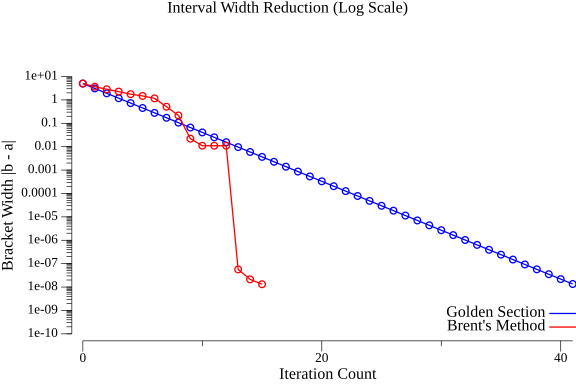
\includegraphics[width=0.75\textwidth]{material/full/output/width_plot.png}
    \caption{区間幅の縮小}
  \end{figure}
\end{frame}

% 比較スライド (3/3: 考察)
\begin{frame}{収束性能の考察}
  \begin{itemize}
    \item 黄金分割法は対数軸で直線的に減衰（線形収束）
    \item Brent法は放物線補間が効き始めると急激に減衰（超線形収束）
    \vspace{1em}
    \item \textbf{結論}:
    \begin{itemize}
      \item Brent法は黄金分割法と比べ、イテレーション数で約 2.6倍高速に収束
      \item 計算時間では約 3.21倍高速に収束
      \item 放物線補間が効率的に機能していることを示す
    \end{itemize}
  \end{itemize}
\end{frame}
